\begin{itemize}
	\item Также находятся параметры $m_{\chi}$ и $\delta$, при которых предположение о равновесии между аннигиляцией и захватом ($\Gamma = \frac{1}{2} C$) перестает быть верным.
\end{itemize}


\begin{figure}[!h]
	\centering
	\only<1>{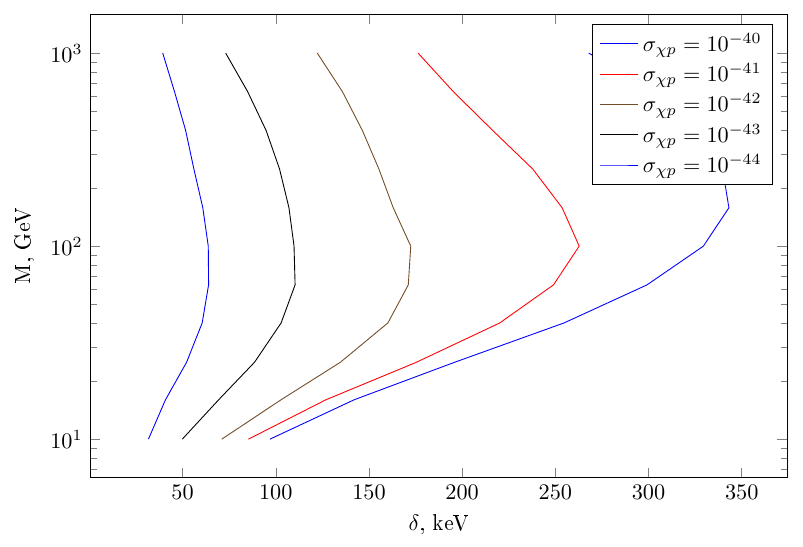
\includegraphics[width=0.6\textwidth]{images/Equilibrium.png}
	\caption{Область параметров $m,\delta$ при которых наступает равновесие между $\Gamma$ и $C$ ($\chi^*$ --- долгоживущая )}
	}
	\only<2>{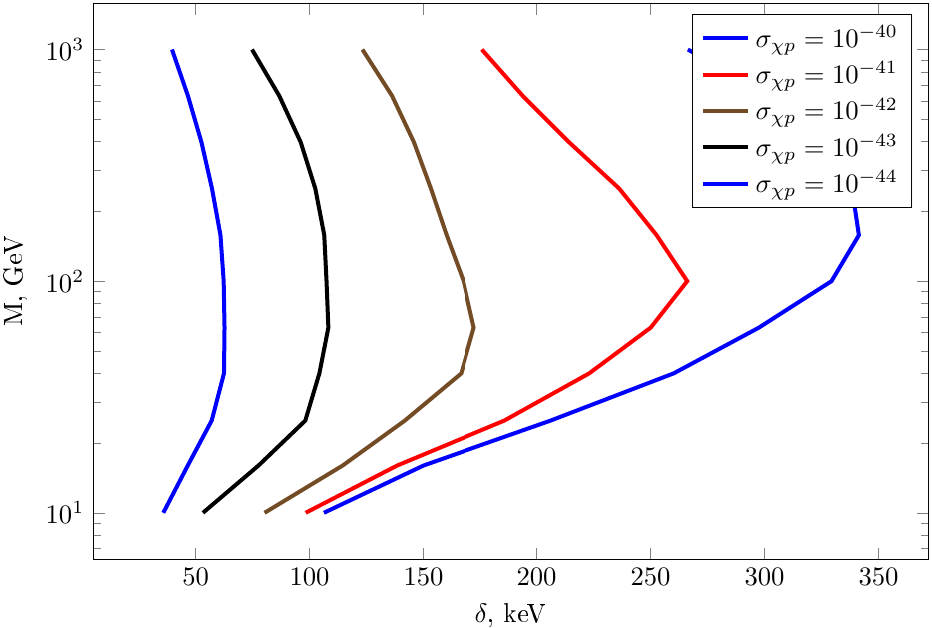
\includegraphics[width=0.6\textwidth]{images/EqFD.png}
	\caption{Область параметров $m,\delta$ при которых наступает равновесие между $\Gamma$ и $C$ ($\chi^*$ --- короткоживущая )}
	}
	
\end{figure}
